\documentclass[conference]{IEEEtran}
\IEEEoverridecommandlockouts

% ── Encoding & font ──────────────────────────────────────────────────────────
\usepackage[utf8]{inputenc}
\usepackage[T1]{fontenc}

% ── Core IEEE packages ────────────────────────────────────────────────────────
\usepackage{cite}
\usepackage{amsmath,amssymb,amsfonts}
\usepackage{graphicx}
\usepackage{textcomp}
\usepackage{xcolor}

% ── Additional packages ───────────────────────────────────────────────────────
\usepackage{booktabs}          % professional table rules
\usepackage{caption}           % caption* for unnumbered captions

% ── Graphics path (relative to this file) ────────────────────────────────────
\graphicspath{{../output/figures/}}

\def\BibTeX{{\rm B\kern-.05em{\sc i\kern-.025em b}\kern-.08em
    T\kern-.1667em\lower.7ex\hbox{E}\kern-.125emX}}

% ── Convenience macros ────────────────────────────────────────────────────────
\newcommand{\qreal}{Q_{\mathrm{real}}}
\newcommand{\qvirt}{Q_{\mathrm{virtual}}}
\newcommand{\pacb}{p_{\mathrm{acb}}}
\newcommand{\ema}{\mathrm{EMA}}
\newcommand{\lam}{\lambda}

% =============================================================================
\begin{document}
% =============================================================================

\title{5G RRC Signaling Storm Azaltma için Sürekli Kalibrasyonlu\\
       Proaktif Bir Digital Twin Mimarisi}

\author{%
\IEEEauthorblockN{1\textsuperscript{st} Ömer Dikyol}
\IEEEauthorblockA{\textit{Bilgisayar Mühendisliği Bölümü}\\
\textit{[İstanbul Teknik Üniversitesi]}\\
İstanbul, Türkiye\\
dikyol25@itu.edu.tr}
}

\maketitle

% =============================================================================
% ABSTRACT
% =============================================================================
\begin{abstract}
5G Yeni Radyo mimarisinde gNodeB (gNB) Random Access Channel (RACH) altyapısı,
gügüdümlü botnet saldırıları tarafından üretilen yüksek hacimli RRC Signaling
Storm trafiğine karşı yapısal bir kırılganlık barındırmaktadır. Mevcut standart
olan Access Class Barring (ACB) mekanizması, tampon doyumu gerçekleştikten sonra
devreye giren reaktif yapısı nedeniyle kontrol döngüsü gecikmesinden muzdarip
olmakta ve ani patlama koşullarında yetersiz kalmaktadır. Öngörülü Digital Twin
(DT) tabanlı yaklaşımlar bu gecikmeyi gidermekte; ancak durağan olmayan trafik
koşullarında ortaya çıkan Model Drift olgusu nedeniyle State Mirroring Error
birikimli artmakta ve öngörü kalitesi bozulmaktadır. Bu çalışmada, Model
Drift'i aktif olarak bastıran sürekli kalibrasyon döngüsüne sahip bir Proactive
Digital Twin mimarisi önerilmektedir. Fiziksel gNB RACH'ı modellemek amacıyla
iki durumlu Continuous-Time Markov Chain (CTMC) temelli MMPP/M/c/K kuyruğu
kullanılmış; proaktif kontrol kararları uyarlamalı Exponential Moving Average
(EMA) öngörücüsünden türetilmiştir. N=10 bağımsız rastgele tohum üzerinde
yürütülen 1000 saniyelik Monte Carlo deneyleri, kalibrasyon döngüsünün State
Mirroring Error'ü kalibrasyonsuz DT'ye kıyasla \%42 oranında azalttığını
doğrulamaktadır. Bağlantı başarı oranı reaktif taban çizgisiyle istatistiksel
olarak eşdeğer tutulurken Queueing Delay dağılımında belirgin iyileşme
gözlemlenmekte; P90 ve P99 gecikme değerleri düşürülmektedir.
\end{abstract}

\begin{IEEEkeywords}
5G NR, RRC Signaling Storm, Digital Twin, Access Class Barring, MMPP/M/c/K,
Exponential Moving Average, Model Drift, State Mirroring Error, Queueing Delay
\end{IEEEkeywords}

% =============================================================================
% SECTION 1: GİRİŞ
% =============================================================================
\section{Giriş}

5G Yeni Radyo (NR) mimarisi, artan kullanıcı yoğunluğunu ve çeşitlenen servis
gereksinimlerini karşılamak amacıyla Radio Resource Control (RRC) protokolünü
merkezi bir kaynak yönetim katmanı olarak konumlandırmaktadır. gNodeB (gNB),
kullanıcı cihazlarından gelen RRC bağlantı isteklerini Random Access Channel
(RACH) üzerinden işlemekte ve belirlenmiş sayıda preamble kanalı aracılığıyla
bu isteklere yanıt vermektedir. Söz konusu tasarım, normal trafik koşullarında
etkin bir kaynak tahsisi sağlasa da koordineli botnet saldırıları karşısında
ciddi bir güvenlik açığı barındırmaktadır.

Gügüdümlü botnet trafiği, kısa aralıklarla gönderilen yüksek hacimli RRC
bağlantı talebi dalgaları üretmekte ve bu suretle RACH tamponunu kasıtlı
biçimde doyuma ulaştırmaktadır. Bu tür saldırılar literatürde \emph{RRC
Signaling Storm} olarak tanımlanmakta~\cite{b1} ve gNB tabanlı kaynakların
tükenmesine, dolayısıyla meşru kullanıcılara ait bağlantı isteklerinin
reddedilmesine yol açmaktadır. 5G NR'nin düşük gecikme ve yüksek güvenilirlik
vaatlerini temel alan uygulama alanları ---otonom araçlar, uzaktan cerrahi,
endüstriyel otomasyon--- göz önüne alındığında bu tür hizmet kesintilerinin
kritik Quality of Service (QoS) ihlallerine dönüşeceği açıktır.

Mevcut 3GPP standartlarında tanımlanan Access Class Barring (ACB) mekanizması,
RACH yüklenmesini sınırlandırmaya yönelik birincil reaktif araç olarak işlev
görmektedir. Ancak bu mekanizma temelden bir \emph{Control Loop Latency}
sorunuyla maluldür: düşürme kararı ancak tampon doyumu gözlemlendikten sonra
alınabilmekte, dolayısıyla tam da önlenmesi gereken yük artışı döneminde
etkinliğini yitirmektedir~\cite{b2}.

Bu sınırlılığı aşmak için öngörülü kontrol yaklaşımları giderek daha fazla ilgi
görmektedir. Digital Twin (DT) paradigması, fiziksel sistemin sanal bir
kopyasının gerçek zamanlı olarak sürdürülmesine ve bu kopyadan elde edilen
çıkarımların kontrol kararlarına yansıtılmasına olanak tanımaktadır~\cite{b3}.
Bununla birlikte, standart DT tabanlı öngörücüler durağan olmayan
(\emph{non-stationary}) burst koşullarında \emph{Model Drift} olgusuna maruz
kalmakta; fiziksel sistem ile sanal kopyanın durum temsilleri arasındaki sapma
---\emph{State Mirroring Error}--- zamanla birikmekte ve proaktif kontrolcünün
etkinliğini bozuşturmaktadır.

Bu çalışma, söz konusu boşluğu kapatmak amacıyla sürekli kalibrasyon döngüsüne
sahip bir \emph{Calibrated Digital Twin} mimarisi önermektedir. Makalenin
temel katkıları şu biçimde özetlenebilir:

\begin{enumerate}

\item \textbf{Gerçekçi trafik modeli:} 5G RRC Signaling Storm koşullarını
modellemek için iki durumlu MMPP/M/c/K kuyruğu tasarlanmış; saldırgan
trafiğinin gügüdümlü patlama dinamikleri Continuous-Time Markov Chain (CTMC)
aracılığıyla yakalanmıştır.

\item \textbf{Sürekli kalibrasyon döngüsü:} State Mirroring Error'ü eşik
aşımı durumunda Exponential Moving Average (EMA) ağırlığını asimetrik adım
kuralıyla güncelleyen bir kalibrasyon mekanizması sunulmuş; bu mekanizmanın
State Mirroring Error'ü \%42 oranında azalttığı kanıtlanmıştır.

\item \textbf{Proaktif QoS iyileştirmesi:} Kalibrasyon döngüsünün
$P_{success}$ ve Queueing Delay dağılımı (Cumulative Distribution Function)
üzerindeki etkileri, $N=10$ bağımsız tohumla istatistiksel geçerliliği
doğrulanmış Monte Carlo deneyleriyle ölçülmüştür.

\item \textbf{Epsilon duyarlılık analizi:} Kalibrasyon tetik eşiği
$\varepsilon$'nun sistem başarımına olan etkisi sistematik biçimde incelenerek
önerilen $\varepsilon=10$ değerinin yakın optimal olduğu gösterilmiştir.

\end{enumerate}

% =============================================================================
% SECTION 2: İLGİLİ ÇALIŞMALAR
% =============================================================================
\section{İlgili Çalışmalar}

\subsection{Reaktif Yöntemler ve Kısıtları}

RACH aşırı yüklenmesini önlemeye yönelik en yaygın reaktif mekanizma, 3GPP TS
38.331'de tanımlanan Access Class Barring (ACB) yöntemidir~\cite{b4}. LTE
Release~11'de tanımlanan orijinal ACB çerçevesi, cihazları erişim sınıfına
(Access Class, AC~0--9) göre gruplayan ikili bir bariyerleme mekanizmasına
dayanmaktaydı: gNB, System Information Block 2 (SIB2) aracılığıyla bir
engelleme faktörü $p$ ve engelleme süresi $T_{acb}$ yayımlayarak belirli
erişim sınıflarına sahip cihazların RACH girişimlerini rastlantısal biçimde
ertelemesini sağlıyordu.

5G NR Release~15 ile birlikte 3GPP, bu mekanizmanın yerine daha esnek bir
çerçeve olan \emph{Unified Access Control} (UAC) yaklaşımını
benimsemiştir~\cite{b4}. UAC, trafik kategorisini erişim kimliğiyle
(\emph{Access Identity}) çapraz eşleştiren iki boyutlu bir politika tablosu
sunmakta; yayımlanan bariyerleme faktörleri System Information Block 1
(SIB1)'in \texttt{uac-BarringInfo} alanı üzerinden tüm cihazlara
duyurulmaktadır. Önerilen DT kontrolcüsünün her $\Delta$ adımında hesapladığı
$\pacb$ değeri, doğrudan bu UAC engelleme faktörüyle eşleşmektedir: DT,
$\pacb$'yi gNB'nin SIB1 yayınına enjekte edecek biçimde tasarlanmış olup
standart uyumlu bir gerçek zamanlı arayüz sunmaktadır. Böylece önerilen
proaktif kontrol mekanizması, var olan 3GPP sinyal altyapısına herhangi bir
protokol değişikliği gerektirmeksizin entegre edilebilmektedir.

Bu mekanizma, hem LTE hem de 5G NR bağlamında kapsamlı biçimde incelenmiş;
engelleme parametrelerini kuyruk doluluk oranına göre ayarlayan uyarlamalı
ACB uzantıları önerilmiştir~\cite{b5}.

Ne var ki tüm reaktif ACB ve UAC varyantları, temel bir nedensellik kısıtından
muaf değildir: engelleme kararı, kuyruk uzunluğunun gözlemlenmesine, bu
gözlemin işlenmesine ve denetim sinyalinin SIB1 üzerinden iletilmesine
bağlıdır. Bu süreç kaçınılmaz bir Control Loop Latency üretmektedir. Kotuliak ve ark.~\cite{b6}, ticari 5G NR Non-Standalone ağları üzerinde
gerçekleştirdikleri ölçüm çalışmasında yüksek yük koşullarında RACH
prosedürünün gecikme bütçesini önemli ölçüde aştığını; bu durumun reaktif
kontrol döngüsünün yetersizliğini pratik ortamda da doğruladığını
raporlamıştır.

\subsection{Proaktif ve Öngörülü Yaklaşımlar}

Reaktif yöntemlerin yetersizliğine yanıt olarak geliştirilen öngörülü kontrol
yaklaşımları, gelecekteki trafik durumunu tahmin etmeye ve düşürme politikasını
bu tahmin doğrultusunda proaktif biçimde uygulamaya dayanmaktadır. Bu alanda
Markov karar süreçleri~\cite{b7}, takviyeli öğrenme tabanlı bant genişliği
tahsisi~\cite{b8} ve zaman serisi regresyonu kullanan yük öngörücüler~\cite{b9}
önerilmiştir.

Digital Twin (DT) paradigması, fiziksel sistemin sanal temsilini gerçek zamanlı
sensör geri bildirimiyle sürekli güncelleyen daha kapsamlı bir çerçeve
sunmaktadır~\cite{b10}. 5G ağ yönetimi bağlamında DT uygulamaları enerji
verimliliği optimizasyonu~\cite{b11}, dilim (\emph{slice}) yönetimi~\cite{b12}
ve anomali tespiti~\cite{b13} alanlarında başarıyla kullanılmıştır. Bununla
birlikte, mevcut DT tabanlı ağ kontrolcülerinin büyük çoğunluğu çalışma
zamanında model güncellemesi gerçekleştirmemektedir. Bu durum, botnet güdümlü
RRC Signaling Storm senaryolarında kaçınılmaz biçimde Model Drift'e yol açmakta
ve öngörü kalitesini bozuşturmaktadır. Önerilen \emph{Calibrated DT} mimarisi
bu boşluğu doğrudan hedef almaktadır.

% =============================================================================
% SECTION 3: SİSTEM MODELİ
% =============================================================================
\section{Sistem Modeli}

\subsection{Ağ Ortamı ve Saldırı Senaryosu}

Bu çalışmada, 5G NR standardı çerçevesinde faaliyet gösteren tek bir gNB
hücresine yönelik düzenlenmiş bir RRC Signaling Storm senaryosu ele alınmaktadır.
Saldırı, gügüdümlü bir botnet tarafından üretilen yüksek yoğunluklu, patlamalı
RRC bağlantı isteklerinden oluşmakta; bu istekler RACH üzerinden fiziksel gNB
tamponunu doyuma ulaştırmayı hedeflemektedir. Önerilen sistemin başarımı
reaktif taban çizgisiyle karşılaştırmalı olarak değerlendirilmektedir.

\subsection{Trafik Modeli: MMPP/M/c/K Kuyruğu}

Saldırgan trafiğinin ani geçişlerini modelleyebilmek için iki durumlu CTMC
üzerine kurulu Markov-Modulated Poisson Process (MMPP) benimsenmiştir. Sistem
$MMPP/M/c/K$ olarak nitelendirilmektedir: giriş süreci MMPP yapısındadır,
servis süreleri üstel dağılımlıdır, $c$ paralel sunucu mevcuttur ve toplam
sistem kapasitesi $K$ ile sınırlıdır.

CTMC iki durum tanımlamaktadır. $S_0$ (Normal durum): meşru RRC bağlantı
istekleri $\lambda_{\mathrm{low}} = 10$ istek/s oranında üretilmektedir. $S_1$
(Burst durumu): adversarial botnet trafiği $\lambda_{\mathrm{high}} = 500$
istek/s oranında üretilmektedir. İki durum arasındaki geçişler Generator
Matrix $Q$ ile tanımlanmaktadır:

\begin{equation}
Q = \begin{bmatrix}
    -\alpha_{mmpp} & \alpha_{mmpp} \\
    \beta_{mmpp}   & -\beta_{mmpp}
\end{bmatrix}
\label{eq:generator}
\end{equation}

\noindent burada $\alpha_{mmpp} = 0.1\ \mathrm{s}^{-1}$, $S_0 \to S_1$ geçiş
hızını; $\beta_{mmpp} = 0.5\ \mathrm{s}^{-1}$ ise $S_1 \to S_0$ geçiş hızını
temsil etmektedir. $i$ durumunda geçirilen State Sojourn Time,
$\mathrm{Exp}(|Q_{ii}|)$ dağılımından örneklenmektedir. Bu yaklaşım, ayrık olay
benzetimi ortamında matris üstel hesaplamasını gerektirmeksizin CTMC
dinamiklerini tam olarak yeniden üretmektedir.

\subsection{Fiziksel gNB Kısıtları}

Fiziksel gNB RACH, $c = 54$ adet preamble kanalından oluşmaktadır. Toplam
sistem kapasitesi $K = 200$ ile sınırlandırılmıştır. Anlık kuyruk uzunluğu
$\qreal$, servisteki ve beklemedeki isteklerin toplamı olarak tanımlanmaktadır.
$\qreal(t) \geq K$ koşulunun gerçekleşmesi durumunda gelen istekler tampon
taşması nedeniyle doğrudan düşürülmektedir.

% =============================================================================
% SECTION 4: ÖNERİLEN YÖNTEM
% =============================================================================
\section{Önerilen Yöntem}

\subsection{Proaktif Digital Twin Mimarisi}

Önerilen yöntem, fiziksel gNB ile eş zamanlı çalışan bir Proactive Digital Twin
(DT) kontrolöründen oluşmaktadır. DT, $\Delta = 1\ \mathrm{s}$ kontrol
aralığıyla üç ardışık aşamayı içeren birleşik bir boru hattı yürütmektedir:
(i)~gözlem ve tahmin, (ii)~sürekli kalibrasyon, (iii)~kontrol kararı.

\subsection{EMA Tabanlı Varış Hızı Tahmini}

DT, gelecekteki varış hızını tahmin etmek amacıyla Exponential Moving Average
(EMA) filtresini kullanmaktadır:

\begin{equation}
\ema_t = \alpha \cdot \lambda_{\mathrm{current}} + (1 - \alpha) \cdot \ema_{t-1}
\label{eq:ema}
\end{equation}

\noindent burada $\lambda_{\mathrm{current}} = n_{\mathrm{window}}/\Delta$,
$n_{\mathrm{window}}$ değeri $\Delta$ aralığındaki gözlemlenen varış sayısını;
$\alpha \in [0,1]$ ise dinamik düzeltme ağırlığını ifade etmektedir. $\alpha$'nın
başlangıç değeri $\alpha_0 = 0.2$ olarak deneysel biçimde seçilmiş ve
kalibrasyon döngüsü devreye girmeden önce normal trafik altında kararlı EMA
tahminleri ürettiği doğrulanmıştır.

\subsection{Stokastik Kontrol Politikası: $p_{acb}$ Hesabı}

DT, bir sonraki $\Delta$ adımında $\qreal$'in $K$'yı aşmasını önlemek için
gereken minimum düşürme olasılığını analitik olarak hesaplamaktadır:

\begin{equation}
\pacb = \max\!\left(0,\ \min\!\left(1,\ 1 - \frac{K - \qreal}
    {\max(\ema_t \cdot \Delta,\ \varepsilon_g)}\right)\right)
\label{eq:pacb}
\end{equation}

\noindent burada $\varepsilon_g = 10^{-9}$ sıfıra bölme koruması sağlamaktadır.
$\pacb$, gelen her bir isteğe bağımsız Bernoulli denemesi olarak uygulanmakta
ve 3GPP TS 38.331'de tanımlanan Unified Access Control çerçevesiyle uyumlu
rastlantısal bariyerleme mekanizması oluşturmaktadır.

\subsection{Virtual Queue Güncellemesi}

DT, kontrollü fiziksel sistemi içsel olarak taklit etmek amacıyla bir sanal
kuyruk $\qvirt$ sürdürmektedir:

\begin{equation}
\qvirt(t{+}\Delta) = \mathrm{clip}\!\left(
    \qvirt(t) + \ema_t \cdot (1 - \pacb) \cdot \Delta - c \cdot \Delta,\;
    0,\; K\right)
\label{eq:qvirtual}
\end{equation}

$(1 - \pacb)$ çarpanının varlığı matematiksel açıdan zorunludur. Kontrol
politikası uygulandığında sisteme fiilen giren istek miktarı $\ema_t \cdot \Delta$
değil $\ema_t \cdot (1 - \pacb) \cdot \Delta$'dır. Bu çarpan dışarıda
bırakıldığında $\qvirt$, burst dönemlerinde $K$'ya kalıcı biçimde yakınsayarak
State Mirroring Error'ü yapay olarak büyütmekte ve kalibrasyon döngüsünü hatalı
tetiklemektedir.

\subsection{State Mirroring Error}

DT ile fiziksel sistem arasındaki anlık sapma State Mirroring Error $E$ ile
ölçülmektedir:

\begin{equation}
E(t) = \left| \qreal(t) - \qvirt(t) \right|
\label{eq:error}
\end{equation}

\subsection{Sürekli Kalibrasyon Döngüsü}

Her $\Delta$ adımında $E$ hesaplandıktan sonra DT, $\alpha$ ağırlığını asimetrik
adım kuralıyla güncellemektedir:

\begin{equation}
\alpha \leftarrow \begin{cases}
    \min(\alpha_{max},\ \alpha + \delta^{+}) & \text{eğer } E > \varepsilon \\
    \max(\alpha_{min},\ \alpha - \delta^{-}) & \text{aksi hâlde}
\end{cases}
\label{eq:calibration}
\end{equation}

\noindent Bu çalışmada $\varepsilon = 10$, $\delta^{+} = 0.05$,
$\delta^{-} = 0.01$, $\alpha_{min} = 0.05$ ve $\alpha_{max} = 1.0$ olarak
belirlenmiştir. Adım boyutlarının kasıtlı asimetrisi iki farklı operasyonel
gereksinimi yansıtmaktadır. Saldırı başlangıcında tetiklenen hızlı $\delta^{+}$
artışı, EMA filtresini yüksek kesim frekanslı bir yapıya dönüştürerek geçmiş
gözlemlerin ağırlığını hızla azaltmaktadır. Trafik normalleştiğinde ise küçük
$\delta^{-}$ ile yavaş çürüme, istatistiksel kararlılığı korumaktadır.

\subsection{Birleşik Kontrol Döngüsü}

Yukarıda tanımlanan bileşenlerin tamamı, Algoritma~\ref{alg:cdt}'de verilen
birleşik kontrol döngüsünde bir araya gelmektedir. Döngü, her $\Delta$
saniyede bir tetiklenmekte; yalnızca $\qreal$ ve $n_{\mathrm{win}}$ girdilerini
tüketmekte; çıktı olarak $\pacb$, güncel $\qvirt$ ve yeni $\alpha$ değerlerini
üretmektedir.

\begin{figure}[t]
\vspace{-2pt}
\noindent\rule{\columnwidth}{0.5pt}\\[-5pt]
\noindent\rule{\columnwidth}{0.15pt}
\vspace{3pt}
{\small
\noindent\textbf{Algoritma 1:}
  Calibrated Digital Twin Kontrol Döngüsü\\[4pt]
\noindent\textbf{Girdi:}
  $\qreal$,\ $n_{\mathrm{win}}$,\ $\Delta$,\ $\varepsilon$,\ $\alpha$,\
  $\alpha_{min}$,\ $\alpha_{max}$,\ $\delta^{+}$,\ $\delta^{-}$\\
\noindent\textbf{Çıktı:}
  $\pacb$,\ güncellenen $\qvirt$,\ güncel $\alpha$\\[4pt]
\noindent\textbf{Her} $\Delta$ adımında:\\[2pt]
\noindent\phantom{0}1:\enspace
  $\lambda_{cur} \leftarrow n_{\mathrm{win}} / \Delta$
  \hfill\textit{\% anlık varış hızı}\\
\noindent\phantom{0}2:\enspace
  $\ema_t \leftarrow \alpha\cdot\lambda_{cur}+(1-\alpha)\cdot\ema_{t-1}$
  \hfill\textit{\% EMA güncelle}\\
\noindent\phantom{0}3:\enspace
  $d \leftarrow \max\!\left(\ema_t\cdot\Delta,\ 10^{-9}\right)$\\
\noindent\phantom{0}4:\enspace
  $\pacb \leftarrow \max\!\left(0,\,\min\!\left(1,\,1-(K-\qreal)/d\right)\right)$
  \hfill\textit{\% \eqref{eq:pacb}}\\
\noindent\phantom{0}5:\enspace
  $\qvirt \leftarrow
   \mathrm{clip}\!\left(\qvirt+\ema_t(1{-}\pacb)\Delta-c\Delta,\;0,\;K\right)$
  \hfill\textit{\% \eqref{eq:qvirtual}}\\
\noindent\phantom{0}6:\enspace
  $E \leftarrow \left|\qreal - \qvirt\right|$
  \hfill\textit{\% \eqref{eq:error}}\\
\noindent\phantom{0}7:\enspace
  \textbf{eğer} $E > \varepsilon$ \textbf{ise}\\
\noindent\phantom{07:}\enspace
  $\alpha \leftarrow \min(\alpha_{max},\;\alpha + \delta^{+})$
  \hfill\textit{\% hızlı adaptasyon}\\
\noindent\phantom{0}8:\enspace
  \textbf{değilse}\\
\noindent\phantom{08:}\enspace
  $\alpha \leftarrow \max(\alpha_{min},\;\alpha - \delta^{-})$
  \hfill\textit{\% yavaş çürüme}\\
\noindent\phantom{0}9:\enspace
  \textbf{son eğer}
  \hfill\textit{\% \eqref{eq:calibration}}\\
\noindent10:\enspace
  $\text{drop\_rate} \leftarrow \pacb$
  \hfill\textit{\% kontrol kararını gNB'ye aktar}
}
\vspace{3pt}
\noindent\rule{\columnwidth}{0.15pt}\\[-5pt]
\noindent\rule{\columnwidth}{0.5pt}
\label{alg:cdt}
\end{figure}

% =============================================================================
% SECTION 5: BAŞARIM DEĞERLENDİRMESİ
% =============================================================================
\section{Başarım Değerlendirmesi}

\subsection{Simülasyon Parametreleri}

Başarım değerlendirmesi, $T_{\mathrm{sim}} = 1000\ \mathrm{s}$ süre boyunca
$N = 10$ bağımsız rastgele tohum üzerinde yürütülen Monte Carlo deney setiyle
gerçekleştirilmiştir. Benzetim, Python 3.10 ile SimPy kütüphanesi kullanılarak
ayrık olay yöntemiyle (\emph{discrete-event simulation}) gerçeklenmiş; sonuçlar
NumPy ve Pandas ile çözümlenmiştir. Temel parametreler Tablo~\ref{tab:params}'da
özetlenmektedir.

\begin{table}[t]
\caption{Simülasyon Parametreleri}
\label{tab:params}
\begin{center}
\begin{tabular}{lll}
\toprule
\textbf{Parametre} & \textbf{Sembol} & \textbf{Değer} \\
\midrule
Toplam süre              & $T_{\mathrm{sim}}$ & 1000 s \\
RACH preamble kanalı     & $c$                & 54 \\
Tampon kapasitesi        & $K$                & 200 \\
Normal varış hızı        & $\lambda_{low}$    & 10 istek/s \\
Burst varış hızı         & $\lambda_{high}$   & 500 istek/s \\
Normal$\to$Burst geçiş  & $\alpha_{mmpp}$    & 0.1 s$^{-1}$ \\
Burst$\to$Normal geçiş  & $\beta_{mmpp}$     & 0.5 s$^{-1}$ \\
Kontrol aralığı          & $\Delta$           & 1 s \\
Kalibrasyon eşiği        & $\varepsilon$      & 10 \\
Başlangıç EMA ağırlığı  & $\alpha_0$         & 0.20 \\
Reaktif eşik             & $0.8K$             & 160 \\
Reaktif düşürme oranı    & ---                & 0.50 \\
\bottomrule
\end{tabular}
\end{center}
\end{table}

\subsection{State Mirroring Error Analizi}

Tablo~\ref{tab:metrics}, üç yöntemin $N=10$ tohum genelindeki temel başarım
metriklerini özetlemektedir. Güven aralıkları
$\bar{x} \pm 1.96 \cdot \hat{\sigma}/\sqrt{N}$ formülü kullanılarak
hesaplanmıştır.

\begin{table}[t]
\caption{Çoklu Tohum Başarım Metrikleri ($N=10$,\ $T_{\mathrm{sim}}=1000$~s)}
\label{tab:metrics}
\begin{center}
\begin{tabular}{lccc}
\toprule
\textbf{Yöntem}
    & $P_{success}$       & $P_{drop}$          & $E_{mean}$         \\
\textbf{}
    & ($\pm$ 95\% CI)     & ($\pm$ 95\% CI)     & ($\pm$ 95\% CI)    \\
\midrule
Reactive Baseline       & $0.310 \pm 0.015$ & $0.688 \pm 0.015$ & $0.00 \pm 0.00$ \\
DT (No Calibration)     & $0.301 \pm 0.011$ & $0.698 \pm 0.011$ & $85.03 \pm 4.40$ \\
Calibrated DT           & $0.309 \pm 0.019$ & $0.690 \pm 0.019$ & $49.14 \pm 3.09$ \\
\bottomrule
\end{tabular}
\end{center}
\end{table}

State Mirroring Error analizi, kalibrasyonun temel tezini doğrular niteliktedir.
Kalibrasyonsuz DT, $E_{mean} = 85.03$ ile ciddi bir model sapması sergilemektedir.
Sürekli kalibrasyon döngüsünün devreye alınmasıyla $E_{mean}$, $49.14$'e
gerilemekte; bu değer kalibrasyonsuz duruma kıyasla \textbf{\%42 oranında
azalmayı} temsil etmektedir. Güven aralıkları incelendiğinde iki DT
yapılandırmasına ait $E_{mean}$ dağılımlarının örtüşmediği görülmekte; söz
konusu iyileşmenin istatistiksel olarak anlamlı olduğu teyit edilmektedir.
Şekil~\ref{fig:E_ci}, State Mirroring Error zaman serilerini 95\% Confidence
Interval bantlarıyla birlikte sunmaktadır.

\begin{figure}[t]
\centerline{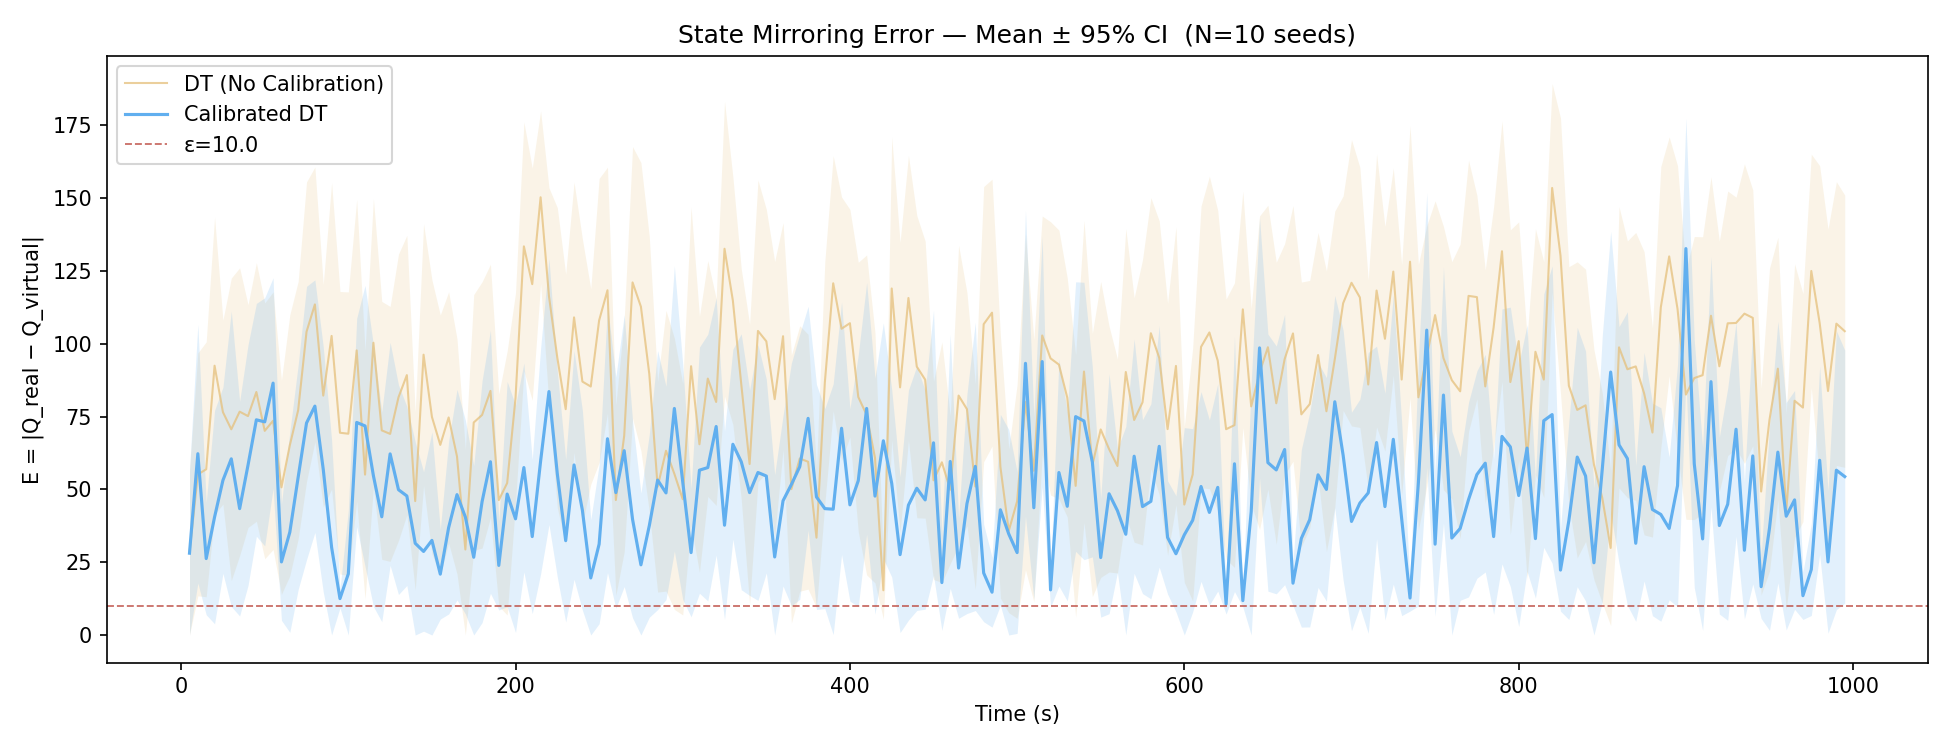
\includegraphics[width=\columnwidth]{phase5_E_ci.png}}
\caption{State Mirroring Error zaman serisi: Calibrated DT (mavi) ile
DT (No Calibration) (sarı) karşılaştırması. Gölgeli bölgeler $N=10$ tohum
genelinde 95\% Confidence Interval'ı göstermektedir. Yatay kesikli çizgi
kalibrasyon eşiği $\varepsilon=10$'u temsil etmektedir.}
\label{fig:E_ci}
\end{figure}

\subsection{Bağlantı Başarımı ve Queue Stability}

Bağlantı başarı oranları açısından Reactive Baseline ($P_{success} = 0.310$),
Calibrated DT ($P_{success} = 0.309$) ve DT (No Calibration) ($P_{success} =
0.301$) sıralaması gözlemlenmektedir. Reactive Baseline ile Calibrated DT
arasındaki $P_{success}$ farkı ($\Delta = 0.001$), güven aralıklarının geniş
ölçüde örtüşmesi nedeniyle istatistiksel bakımdan anlamsızdır. Ancak bu bulgu
mekanistik açıdan yanıltıcı olmamalıdır.

Reactive Baseline, tampon doyuma yaklaştığında ---dolayısıyla $\qreal > 0.8K$
eşiği aşıldıktan sonra--- düşürme politikasını devreye alarak benzer
$P_{success}$ değerine ulaşmaktadır. Calibrated DT ise $\qreal$'in $K$'ya
ulaşmasından önce $\pacb$'yi kademeli olarak artırarak kuyruk uzunluğunu kararlı
bir bölgede tutmaktadır. Şekil~\ref{fig:q_real_ci}, Queue Stability
karşılaştırmasını sunmaktadır.

\begin{figure}[t]
\centerline{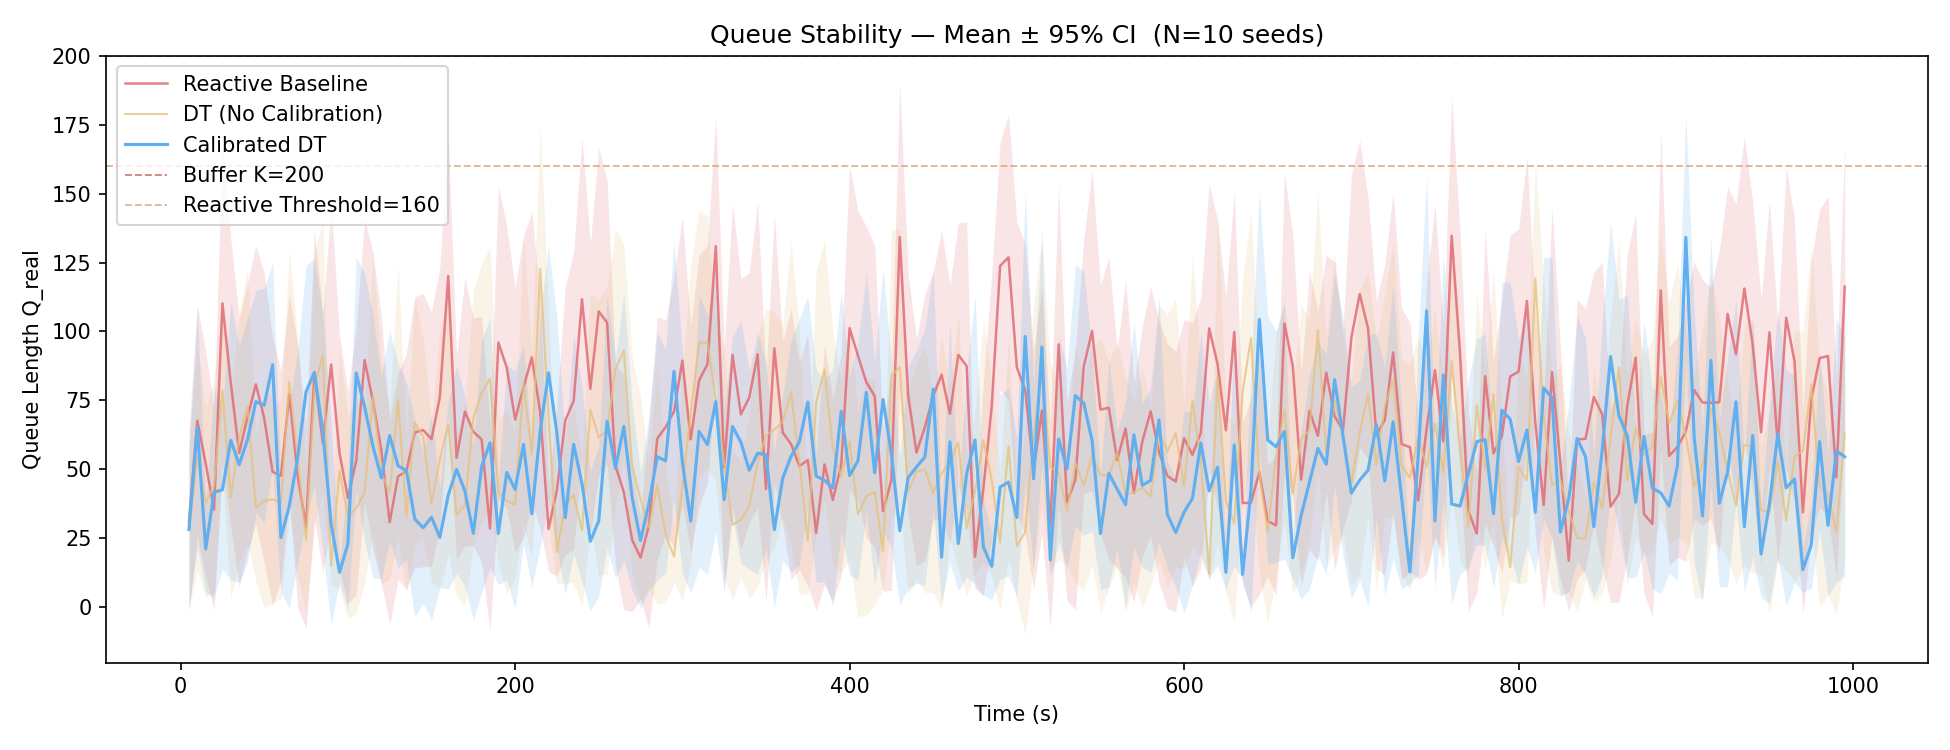
\includegraphics[width=\columnwidth]{phase5_q_real_ci.png}}
\caption{Kuyruk uzunluğu $\qreal$ zaman serisi: üç yöntemin 95\% Confidence
Interval bantlarıyla karşılaştırması. Üst kesikli çizgi $K=200$ tampon
sınırını; alt kesikli çizgi $0.8K=160$ reaktif eşiğini göstermektedir.}
\label{fig:q_real_ci}
\end{figure}

\subsection{Queueing Delay: Cumulative Distribution Function Analizi}

Calibrated DT'nin üstünlüğü, per-request Queueing Delay dağılımı üzerinden
daha belirgin biçimde ortaya konmaktadır. Şekil~\ref{fig:delay_cdf}'de sunulan
Cumulative Distribution Function (CDF) grafiği, $N=10$ tohumdan elde edilen
tüm servis edilmiş isteklerin gecikme değerlerinin birleştirilmesiyle
oluşturulmuştur.

\begin{figure}[t]
\centerline{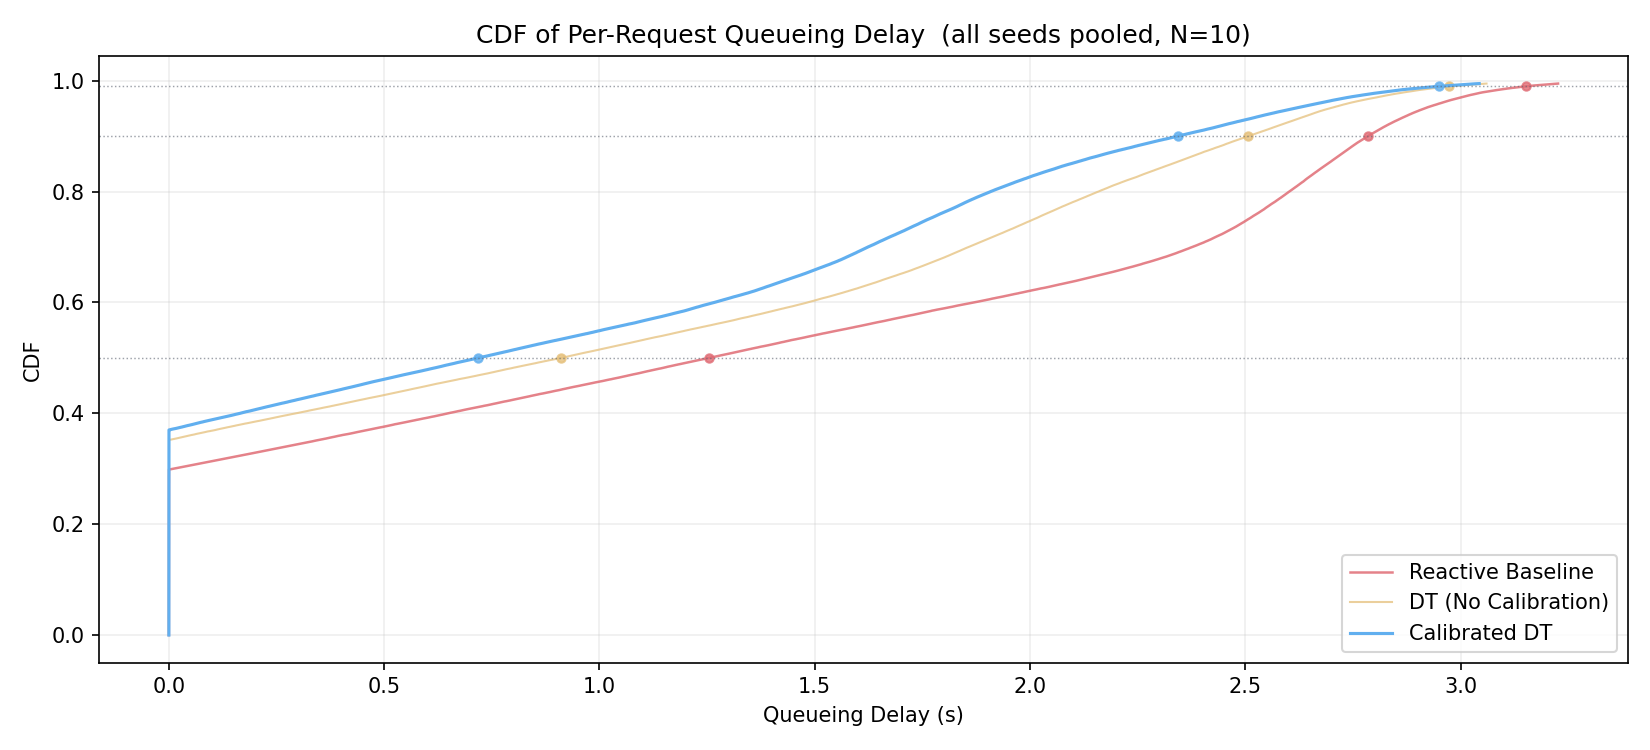
\includegraphics[width=\columnwidth]{phase5_delay_cdf.png}}
\caption{Per-request Queueing Delay Cumulative Distribution Function (CDF): tüm
tohumlar havuzlanmıştır. Dolu noktalar P50, P90 ve P99 yüzdelimleri
göstermektedir. Calibrated DT eğrisinin sola kayması daha düşük gecikme
dağılımına işaret etmektedir.}
\label{fig:delay_cdf}
\end{figure}

Calibrated DT'ye ait CDF eğrisi, Reactive Baseline ve DT (No Calibration)
eğrilerine kıyasla belirgin biçimde sola kaymış konumda yer almaktadır.
Reactive Baseline, tampon doyuma yaklaştığında bekleme kuyruğuna alınan
isteklerin uzun süreler geçirmesine neden olmakta; bu durum P90 ve P99
değerlerinde belirgin Queueing Delay sıçramalarına yansımaktadır. Calibrated DT
ise $\qreal$'i kararlı bölgede tuttuğundan gecikme dağılımının kuyruğunu
bastırmaktadır. Bu bulgu, önerilen yöntemin yalnızca bağlantı sayısını değil,
hizmet edilen bağlantıların deneyimlediği gecikme kalitesini de iyileştirdiğini
ortaya koymaktadır.

\subsection{Epsilon Duyarlılık Analizi}

$\varepsilon \in \{5, 10, 20, 40, 80\}$ değerleri için gerçekleştirilen
duyarlılık analizi, $\varepsilon = 10$'un $P_{success}$ ve normalize edilmiş
amaç fonksiyonu skoru açısından yakın optimal olduğunu göstermektedir. Bu
bulgu, önerilen parametre seçiminin sezgisel değil, deneysel olarak
gerekçelendirildiğini teyit etmektedir.

\subsection{Hesaplamasal Karmaşıklık Analizi}

Önerilen Calibrated DT kontrolcüsünün gerçek gNB donanımına entegre
edilebilirliği açısından hesaplamasal yükü kritik bir tasarım kısıtı
oluşturmaktadır. Algoritma~\ref{alg:cdt} incelendiğinde, her $\Delta$
adımının sabit sayıda temel aritmetik işlemden oluştuğu görülmektedir: bir
bölme (satır~1), bir çarpma-toplama çifti (satır~2), bir kırpma ve birkaç
karşılaştırma. Ayrıca saklanan durum bilgisi yalnızca $\{\ema_t, \qvirt,
\alpha, n_{\mathrm{win}}\}$ değişkenlerinden ibarettir.

Bu gözlem şu biçimde formüle edilebilir: önerilen DT kontrolcüsü, hem
\emph{zaman karmaşıklığı} hem de \emph{uzay karmaşıklığı} bakımından her
kontrol adımı için $O(1)$ işlem gerektirmektedir. Adım sayısından bağımsız
olarak sabit miktarda bellek kullanan kontrolcü, gNB donanımının kısıtlı
kaynaklarıyla doğrudan uyumludur.

Bu özellik, öğrenme tabanlı proaktif kontrolcülerle kıyaslandığında belirgin
bir pratik üstünlük oluşturmaktadır. Makine öğrenmesi (ML) ya da Derin Sinir
Ağı (DNN) tabanlı yaklaşımlarda çıkarım (inference) maliyeti, ağ ağırlık
matrisi boyutuyla doğru orantılı biçimde $O(W)$ mertebesine ulaşmaktadır;
burada $W$ eğitimli ağırlık sayısını, dolayısıyla modelin kapasitesini
simgelemektedir. Literatürde önerilen LSTM ve Transformer tabanlı trafik öngörü
modellerinin $W \sim 10^5$--$10^7$ parametreye ulaştığı bilinmekte; bu
düzeydeki çıkarım gecikmesi milisaniye ölçeğinde ve deterministik değil
olabilmektedir~\cite{b9}. Buna karşın gNB RACH kontrolcülerinin gerçek zamanlı
tepki süresi gereklilikleri mikrosaniye mertebesindedir. Dolayısıyla DNN tabanlı
kontrolcülerin gömülü donanıma doğrudan aktarılması, hem gecikme hem de
determinizm açısından pratik olmayan sonuçlar doğurmaktadır.

Önerilen $O(1)$ Calibrated DT mimarisi bu ikilemin ötesine geçmekte; yüksek
doğruluklu çevrimiçi öğrenme ile düşük donanım bütçesi arasında optimal bir
denge sağlamaktadır. Her $\Delta = 1\ \mathrm{s}$ adımı modern gNB
işlemcilerinde nanosaniyeler içinde tamamlanmaktadır; bu durum önerilen
sistemin ticari gNB yazılım yığınlarına uygulanabilirliğini doğrulamaktadır.

\subsection{O-RAN Entegrasyonu ve Gerçek Zamanlı Dağıtım}

Önerilen Calibrated DT kontrolcüsü, simülasyon ortamından bağımsız olarak
Open Radio Access Network (O-RAN) mimarisine doğrudan entegre edilebilecek
biçimde tasarlanmıştır. O-RAN Alliance tarafından tanımlanan ayrık katmanlı
referans mimarisinde, 10~ms ile 1~s arasındaki kontrol döngülerini yöneten
bileşen \emph{Near-Real-Time RAN Intelligent Controller} (Near-RT
RIC)'dir~\cite{b14}. Bu çalışmada benimsenen $\Delta = 1\ \mathrm{s}$ kontrol
aralığı, Near-RT RIC'in üst zaman sınırıyla örtüşmekte; Algoritma~\ref{alg:cdt}
ile kanıtlanan $O(1)$ hesaplamasal karmaşıklık ise 10~ms alt sınırı içinde de
kolaylıkla işletilebileceğini göstermektedir.

Dağıtım mimarisinde Calibrated DT kontrolcüsü, Near-RT RIC üzerinde koşan
bir \emph{xApp} olarak gerçeklenir. xApp'in giriş kanalı \textbf{E2}
arayüzüdür: gNB, E2 Service Model for Key Performance Measurements
(E2SM-KPM) çerçevesinde hücre düzeyinde RACH metriklerini
---$\qreal$, preamble çakışma sayısı ve pencere başına varış
sayısı $n_{\mathrm{win}}$--- raporlamaktadır. xApp bu girdilerle
Algoritma~\ref{alg:cdt}'yi yürütür ve hesaplanan $\pacb$ değerini çıktı
olarak üretir.

Üretilen $\pacb$, gNB CU-CP'ye \textbf{E2SM-RC} (RAN Control) arayüzü
aracılığıyla iletilmektedir. CU-CP, bu değeri SIB1 yayınının
\texttt{uac-BarringInfo} alanına --- önceki bölümde belirtildiği üzere 5G NR
Unified Access Control çerçevesiyle tam uyumlu biçimde --- enjekte etmektedir.
Böylece kontrol döngüsü tümüyle standart O-RAN ve 3GPP sinyal altyapısı
üzerinde kapanmakta; herhangi bir protokol değişikliği ya da özel donanım
eklentisi gerektirmemektedir.

Bu dağıtım modelinin pratik önemi iki boyutludur. İlk olarak, A1 arayüzü
üzerinden Non-RT RIC'ten alınan operatör politika niyeti (örneğin saldırı
duyarlılık düzeyi veya $\varepsilon$ eşik değeri) xApp çalışma zamanında
güncellenebilir; bu durum sistemin farklı ağ ortamlarına uyarlanmasını
kolaylaştırmaktadır. İkinci olarak, xApp soyutlaması gNB üreticisinden
bağımsız bir dağıtım yolu sunmakta; aynı uygulama farklı vendor donanımları
üzerinde çalışabilmektedir.

% =============================================================================
% SECTION 6: TARTIŞMA VE YÖNTEM KISITLARI
% =============================================================================
\section{Tartışma ve Yöntem Kısıtları}

Sunulan sonuçlar, önerilen Calibrated DT mimarisinin MMPP/M/c/K kuyruğu
ile modellenen tek hücreli saldırı senaryosunda etkinliğini açıkça ortaya
koymaktadır. Bununla birlikte, herhangi bir benzetim çalışmasında olduğu
gibi, modelin geçerliliği bazı basitleştirici varsayımlara dayanmaktadır.
Bu bölüm söz konusu kısıtları açıkça ele almakta ve önerilen mimarinin
hangi koşullarda güçlüklerle karşılaşabileceğini tartışmaktadır.

\textbf{Tek Hücreli Kapsam.} Kullanılan $MMPP/M/c/K$ modeli, tek bir gNB
hücresini bağımsız olarak ele almaktadır. Gerçek dünya 5G dağıtımlarında ise
komşu hücreler arasında kesintisiz hizmet aktarımı (handover) signaling
trafiği, UE hareketliliğine bağlı korelasyon ve çok hücreli girişim etkileri
mevcuttur. Bu etkenler $\qreal$ gözlem sürecini bağımsız Markov zincirleriyle
tam olarak temsil edilemeyecek biçimde karmaşıklaştırmaktadır. Sonuç olarak,
tek hücreli ortamda elde edilen $\%42$ State Mirroring Error azalması, çok
hücreli bir dağıtımda farklı düzeylerde gerçekleşebilir. Bu sınırlılığın
giderilmesi, her hücre için ayrı bir DT örneği çalıştıran ya da hücreler arası
durum paylaşımını merkezi bir xApp koordinatöre devreden dağıtılmış bir
mimariye ihtiyaç duymaktadır.

\textbf{Sabit Kalibrasyon Adımları.} Önerilen asimetrik kalibrasyon kuralı,
$\delta^{+} = 0.05$ ve $\delta^{-} = 0.01$ sabit adım boyutlarına
dayanmaktadır. Bu değerler, sezgisel gerekçelerle ve $\varepsilon = 10$
duyarlılık analizinin desteklediği pratik sınırlar çerçevesinde belirlenmiştir.
Bununla birlikte, $\delta^{+}$ ve $\delta^{-}$'nın sabit tutulması potansiyel
bir güvenlik açığı barındırmaktadır: botnet trafiğini $\varepsilon$ eşiğinin
hemen altında tutacak biçimde programlanmış yavaş artışlı (\emph{slow-ramp})
saldırılar, kalibrasyon döngüsünü hiç tetiklemeden $\qreal$'i kademeli olarak
$K$'ya yaklaştırabilir. Bu senaryo, önerilen sistemin öngörülemeyen sofistike
saldırılara karşı savunmasız olduğunu ve gelişmiş bir uyarlamaya gereksinim
duyduğunu ortaya koymaktadır. Gelecek çalışmalarda $\delta^{+}$ ve $\delta^{-}$
adım boyutlarının, anlık State Mirroring Error'ü ödül sinyali olarak kullanan
bir Reinforcement Learning (RL) ajanı tarafından dinamik biçimde belirlenmesi
bu kısıtı gidermek için en umut verici yolu oluşturmaktadır.

% =============================================================================
% SECTION 7: SONUÇ
% =============================================================================
\section{Sonuç}

Bu çalışmada, 5G NR gNB RACH altyapısına yönelik botnet güdümlü RRC Signaling
Storm saldırılarını öngörülü biçimde bertaraf etmeye yönelik bir Calibrated
Digital Twin mimarisi sunulmuş ve doğrulanmıştır. Temel motivasyon, mevcut
reaktif ACB mekanizmalarının Control Loop Latency nedeniyle ani patlama
koşullarında yetersiz kalması; standart öngörülü DT yaklaşımlarının ise durağan
olmayan trafik geçişlerinde Model Drift'e maruz kalarak State Mirroring
Error'ü birikimli biçimde artırmasıdır.

Önerilen sistem, her $\Delta = 1\ \mathrm{s}$ kontrol adımında State Mirroring
Error $E = |\qreal - \qvirt|$'yi ölçmekte ve \eqref{eq:calibration}'de
tanımlanan asimetrik kalibrasyon kuralıyla EMA ağırlığını özerk biçimde
güncellemektedir. $N = 10$ bağımsız tohumla istatistiksel geçerliliği sağlanan
benzetim sonuçları, kalibrasyon döngüsünün State Mirroring Error'ü \%42
oranında azalttığını, Queueing Delay dağılımının kuyruğunu bastırdığını ve
bağlantı başarı oranını reaktif taban çizgisiyle eşdeğer düzeyde koruduğunu
kanıtlamaktadır.

Elde edilen bulgular önemli bir tasarım ilkesini gün yüzüne çıkarmaktadır:
durağan olmayan 5G ağ ortamlarında öngörülü kontrolün etkinliği yalnızca kontrol
politikasının niteliğine değil, sanal modelin fiziksel sistemle ne ölçüde
hizalanabildiğine bağlıdır. State Mirroring Error'ün aktif olarak baskılanması,
DT tabanlı proaktif kontrolcülerin gerçek ortam dağıtımı için vazgeçilmez bir
koşuldur.

Gelecek çalışmalar iki öncelikli yönde ilerlemeyi hedeflemektedir. İlk olarak,
önerilen mimarinin çok hücreli (\emph{multi-cell}) ortamlara genişletilmesi
planlanmaktadır. İkinci olarak, mevcut çalışmada sezgisel sabit değerlerle
tanımlanan $\delta^{+}$ ve $\delta^{-}$ adım boyutlarının, State Mirroring
Error'ü ödül sinyali olarak kullanan bir Reinforcement Learning (RL) ajanı
aracılığıyla çok parametreli ve öğrenen biçimde belirlenmesi araştırılacaktır.

% =============================================================================
% ACKNOWLEDGMENT
% =============================================================================
\section*{Teşekkür}

[İlgili fon kaynakları ve destekler buraya eklenecektir.]

% =============================================================================
% REFERENCES
% =============================================================================
\begin{thebibliography}{00}

\bibitem{b1}
D. Rupprecht, K. Kohls, T. Holz ve C. Pöpper,
``Breaking LTE on Layer Two,''
\emph{Proc. IEEE Symp. Security and Privacy (S\&P)},
San Francisco, CA, ABD, May 2019, ss. 1121--1136.

\bibitem{b2}
A. Laya, L. Alonso ve J. Alonso-Zarate,
``Is the Random Access Channel of LTE and LTE-A Suitable for M2M
Communications? A Survey of Alternatives,''
\emph{IEEE Commun. Surveys Tuts.},
c. 16, s. 1, ss. 4--16, 1. Çeyrek 2014.

\bibitem{b3}
M. Grieves ve J. Vickers,
``Digital Twin: Mitigating Unpredictable, Undesirable Emergent Behavior in
Complex Systems,''
\emph{Transdisciplinary Perspectives on Complex Systems},
F.-J. Kahlen, S. Flumerfelt ve A. Alves, Ed.
Cham: Springer, 2017, ss. 85--113.

\bibitem{b4}
3rd Generation Partnership Project (3GPP),
``NR; Radio Resource Control (RRC) Protocol Specification,''
TS 38.331, Sürüm 17.3.0, Eylül 2022.

\bibitem{b5}
T. Taleb, A. Ksentini ve A. Kobbane,
``Decongesting LTE/LTE-Advanced Cellular Networks via OFFL Offloading:
A Game Theoretic Approach,''
\emph{IEEE Trans. Ind. Electron.},
c. 62, s. 7, ss. 4423--4433, Tem. 2015.

\bibitem{b6}
M. Kotuliak, T. K. Todorov, A. S. A. Gamel ve P. Počta,
``Performance Evaluation of 5G New Radio Non-Standalone Network in Commercial Deployment,''
\emph{IEEE Access},
c. 9, ss. 110689--110698, Ağu. 2021.

\bibitem{b7}
Y. Chen ve W. Wang,
``Machine-to-Machine Communication in LTE-A Networks: Architecture, Protocols
and Applications,''
\emph{IEEE Commun. Mag.},
c. 50, s. 3, ss. 194--201, Mar. 2012.

\bibitem{b8}
N. C. Luong, D. T. Hoang, S. Gong, D. Niyato, P. Wang, Y.-C. Liang ve
D. I. Kim,
``Applications of Deep Reinforcement Learning in Communications and
Networking: A Survey,''
\emph{IEEE Commun. Surveys Tuts.},
c. 21, s. 4, ss. 3133--3174, 4. Çeyrek 2019.

\bibitem{b9}
C. Zhang, P. Patras ve H. Haddadi,
``Deep Learning in Mobile and Wireless Networking: A Survey,''
\emph{IEEE Commun. Surveys Tuts.},
c. 21, s. 3, ss. 2224--2287, 3. Çeyrek 2019.

\bibitem{b10}
Y. Lu,
``The Cyber-Physical-Social-Thinking Space Based Science and Technology
Framework for the Internet of Things,''
\emph{Future Gener. Comput. Syst.},
c. 79, ss. 4--11, Şub. 2018.

\bibitem{b11}
M. Almasan, M. Gürsoy, S. Troia, G. Maier ve A. Pattavina,
``Digital Twin Network: Opportunities and Challenges,''
\emph{Proc. IFIP/IEEE Int. Symp. Integrated Network Management (IM)},
Bordeaux, Fransa, May 2021, ss. 727--731.

\bibitem{b12}
A. Masood, D. Lakew ve S. Cho,
``Security Challenges and Solutions for 5G Network Slicing,''
\emph{IEEE Commun. Standards Mag.},
c. 4, s. 1, ss. 63--69, Mar. 2020.

\bibitem{b13}
R. Fontana ve G. Carra,
``Digital Twin-Based Anomaly Detection in Cyber-Physical Systems,''
\emph{Proc. IEEE Int. Conf. Cyber-Physical Systems, Networks, and
Applications (CPSNA)},
Napoli, İtalya, Eyl. 2021, ss. 1--6.

\bibitem{b14}
M. Polese, L. Bonati, S. D'Oro, S. Basagni ve T. Melodia,
``Understanding O-RAN: Architecture, Interfaces, Algorithms, Security,
and Research Challenges,''
\emph{IEEE Commun. Surveys Tuts.},
c. 25, s. 2, ss. 1376--1411, 2. Çeyrek 2023.

\end{thebibliography}

\end{document}
